\section{Background}
\label{ch-introduction:sec:background}

% - Background
%   - Electricity grid
%   - Role of energy storage - a survey

Today's society and economy are highly dependent on the continuous availability of energy, or more specifically: electric energy.
Demand for electricity has increased over the past decades, and this trend is expected to continue into the future \cite{HMGovernment2009}.
This demand increase is only accelerated since major focus of UK energy policies has been put on transitioning towards a low carbon economy \cite{RoyalAcademyofEngineering2010}.
Particularly the decarbonisation of heat and transport sectors are two areas of significant strategic focus and Low Carbon Technology (LCT) such as Photo-Voltaic (PV) installations, electric vehicles and heat pumps are expected to contribute significantly to this transition.

However, as adaptation of these LCTs increases and they start to penetrate power distribution networks, stress on these networks will continue to increase even further, which may result in additional service disruptions.
Furthermore, the uptake of LCTs is not expected to progress evenly throughout the entire power network, and instead clusters of early adopters are predicted to form, leading to certain Low-Voltage (LV) networks to exceed their operational constraints even at relatively low national rate of LCT adaption \cite{Poghosyan2014}.
The scale of this energy transition becomes becomes particularly apparent when referring to the UK's future energy scenarios that compare the predicted future load scenarios.

\begin{figure}\centering
	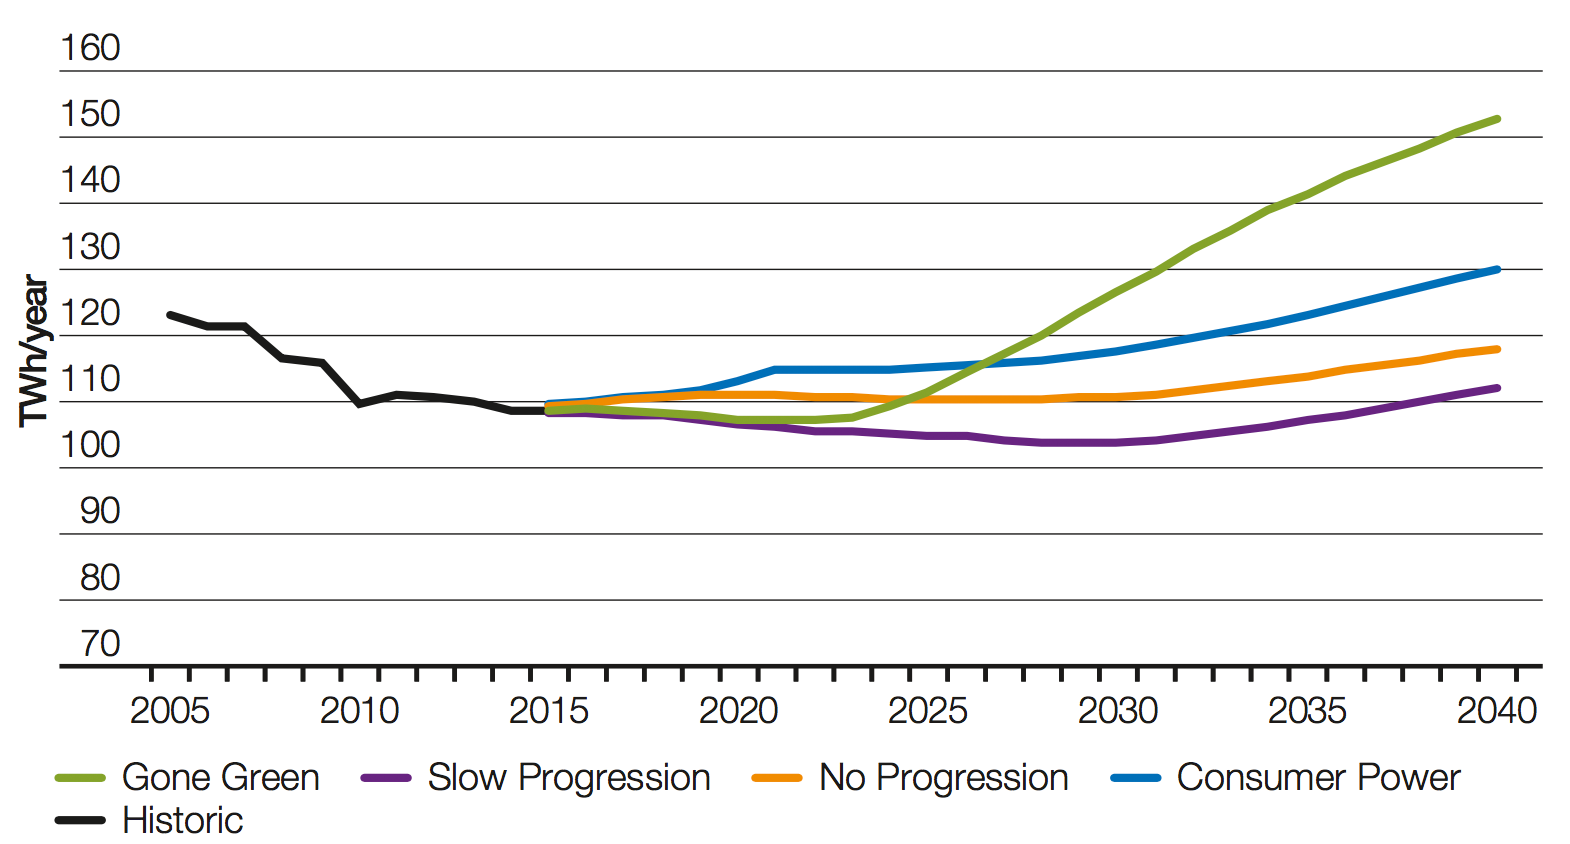
\includegraphics{_introduction/fig/electricity-demand-forecast}
	\caption{Annual residential demand for electricity from FES2016 \cite{FES2016}}
	\label{ch-introduction:fig:electricity-demand-forecast}
\end{figure}

Figure \ref{ch-introduction:fig:electricity-demand-forecast} shows the predicted increase in demand for electric energy when following the UK's 2020 and 2050 goals in reducing green-house emissions.
According to this projection, the annual energy demand will increase by more than 40THh by the year 2040, if the ``Gone Green'' approach is implemented.
This trend is expected despite increasing device efficiencies, since the shift from oil and gas to electricity, i.e. the electrification, offset these gains.

\begin{figure}\centering
	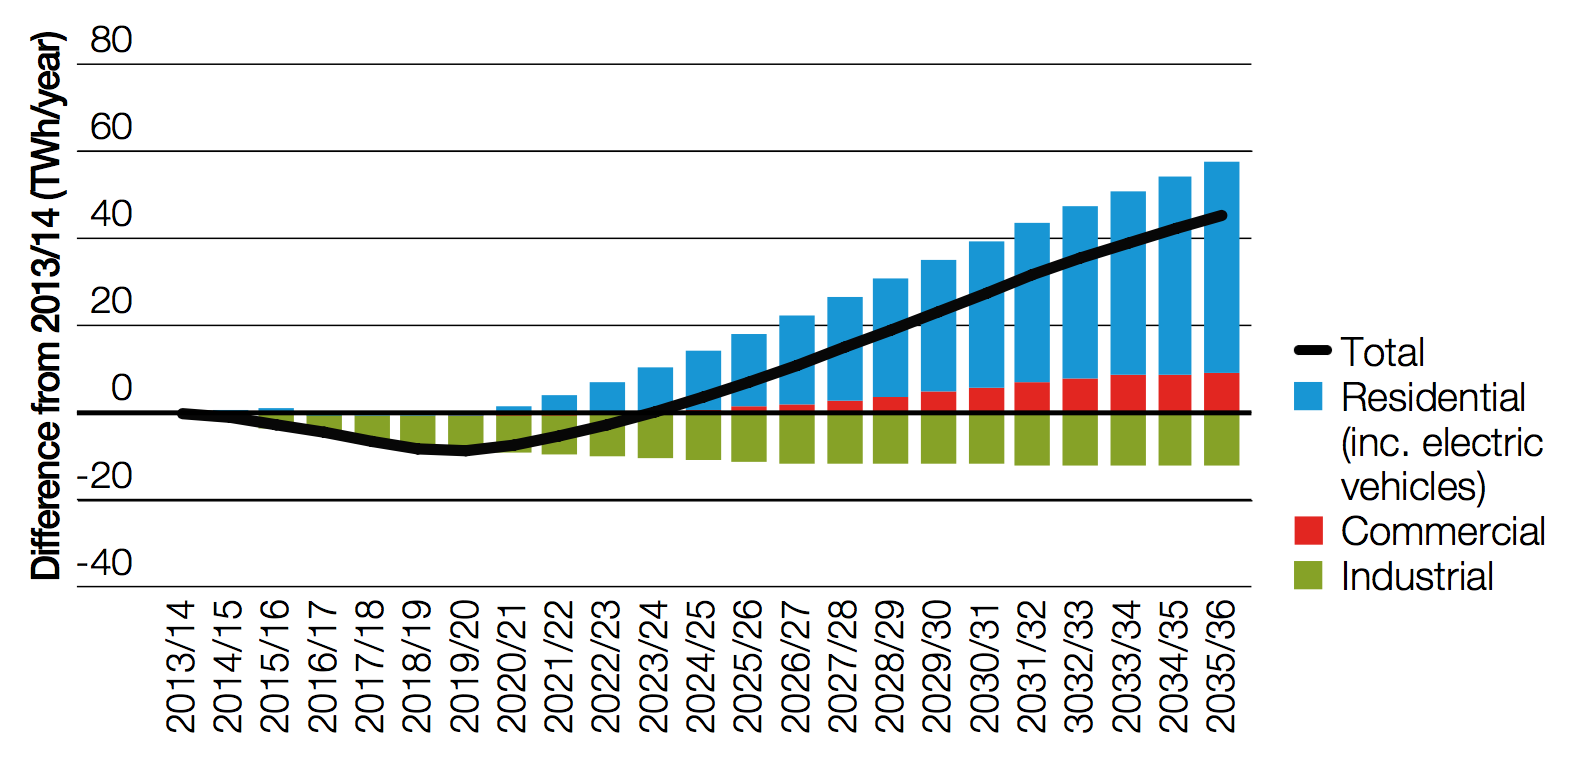
\includegraphics{_introduction/fig/electricity-demand-change-forecast}
	\caption{``Gone Green'' power demand comparison to 2013/14 by type (excluding losses) from FES2015 \cite{FES2015}}
	\label{ch-introduction:fig:electricity-demand-change-forecast}
\end{figure}

When breaking down the change in demand for electricity, as done in Figure \ref{ch-introduction:fig:electricity-demand-change-forecast}, one can observe how industry sectors are expected to decrease energy consumption, yet the residential and commercial sectors will dominantly increase their demand.
To make things worse, those two sectors are typically situated at the network edge, i.e. in the LV distribution network.
This part of the network is its weakest part, since its assets were designed to caters for small powers between 315kVA to 500kVA \cite{EDS08-0115}.
Therefore, strict regulation is in place to assure continuous operation without violating any operating constraints. 

Traditional network planning approaches, that were used to circumvent constraint violations, follow the commonly used practice of aggregating a large number of customers and designing the power delivery network to cater for their largest probable demand, i.e. the After Diversity Maximum Demand (ADMD) method \cite{Richardson2010a}.
This ADMD method has remained the same for many years and uses historical load analysis and standard growth assumptions that are both no longer valid in this unprecedented LCT uptake scenario \cite{Yunusov2016}.
To make things worse, LV networks in the UK are generally unmonitored once installed.
Distribution Network Operators (DNOs) have become aware of this issue and are developing updated planning strategies involving ``smart'' and ``flexible'' electricity grids \cite{Fang2012}.
However, in situ equipment that will become subject to the same adaptation of LCT needs to be managed actively via innovation in the use of existing and new technologies; otherwise both frequency of service disruptions and customer minutes lost will increase alongside the proliferation of LCTs \cite{Ault2008a}.

\subsection{Solutions to mitigate impact of LCT}
\label{ch-introduction:subsec:solutions-to-mitigate-impact-of-lct}

Two solutions exist, allowing DNOs to support LV network's operation: 
\begin{enumerate*}
	\item reinforcement of in situ network assets;
	\item deployment of network support equipment.
\end{enumerate*}
Whilst network reinforcement would certainly address immediate issues of current network capacity constraints, it is also the more expensive and disruptive option.
More specifically, customer will need to deal with outages during periods of asset upgrades (e.g. transformer upgrade and line re-conductoring after secondary transformers' tap settings have been adjusted).
Therefore, alternatives to defer or avoid network reinforcements have been sought and assessed \cite{Harrison2007, Zangs2016a, VanderKlauw2016d, Greenwood2017}.
Most promising alternatives are to install flexible and controllable Distributed Energy Resources (DERs), or more specifically: Battery Energy Storage Solutions (BESS) \cite{Wade2010}.
BESS has not only seen significant advancements in technology, but also received increasing attention in both academic studies and industry trials \cite{Palizban2016}.

Installing BESS on a strategic location in the LV network brings several advantages to DNOs' control over the network's performance.
Roles for BESS are addressed in the subsequent section, i.e. Section \ref{ch-introduction:subsec:role-of-energy-storage-a-survey}.
However, a few examples of potential benefits from BESS include the regulation of voltages to stay within statutory operating bands \cite{Yang2014}, shaving peak loads to relieve stress from the installed network assets \cite{Bennett2015}, and reducing phase unbalance to increase network efficiency \cite{Wang2015b} .
Whilst the questions regarding locating and scaling of BESS have mostly been addressed, BESS control can be split into two complementing yet unmarried approaches:

\begin{enumerate}
	\item ``off-line'' control, using load forecasts and BESS schedules, and
	\item ``on-line'' control, using Set-Points Control (SPC), Model Predictive Control (MPC) or similar dynamic control methods.
\end{enumerate}

Furthermore, with the anticipated uptake of household BESS, mechanisms to control several storage systems also need to be considered.
For instance, several industry leaders propose to store solar energy in order to support charging of EVs \cite{Baumann2017}.
Without rooftop PV installations, batteries need work in a cooperative manner to not impose additional strain onto the network.
The full review of storage control strategies to achieve both off-line and on-line, as well as centralised/individual and distributed battery control is presented in Section \ref{ch-literature:sec:control-of-energy-storage}.

\subsection{Role of energy storage - a survey}
\label{ch-introduction:subsec:role-of-energy-storage-a-survey}


\begin{figure}\centering
	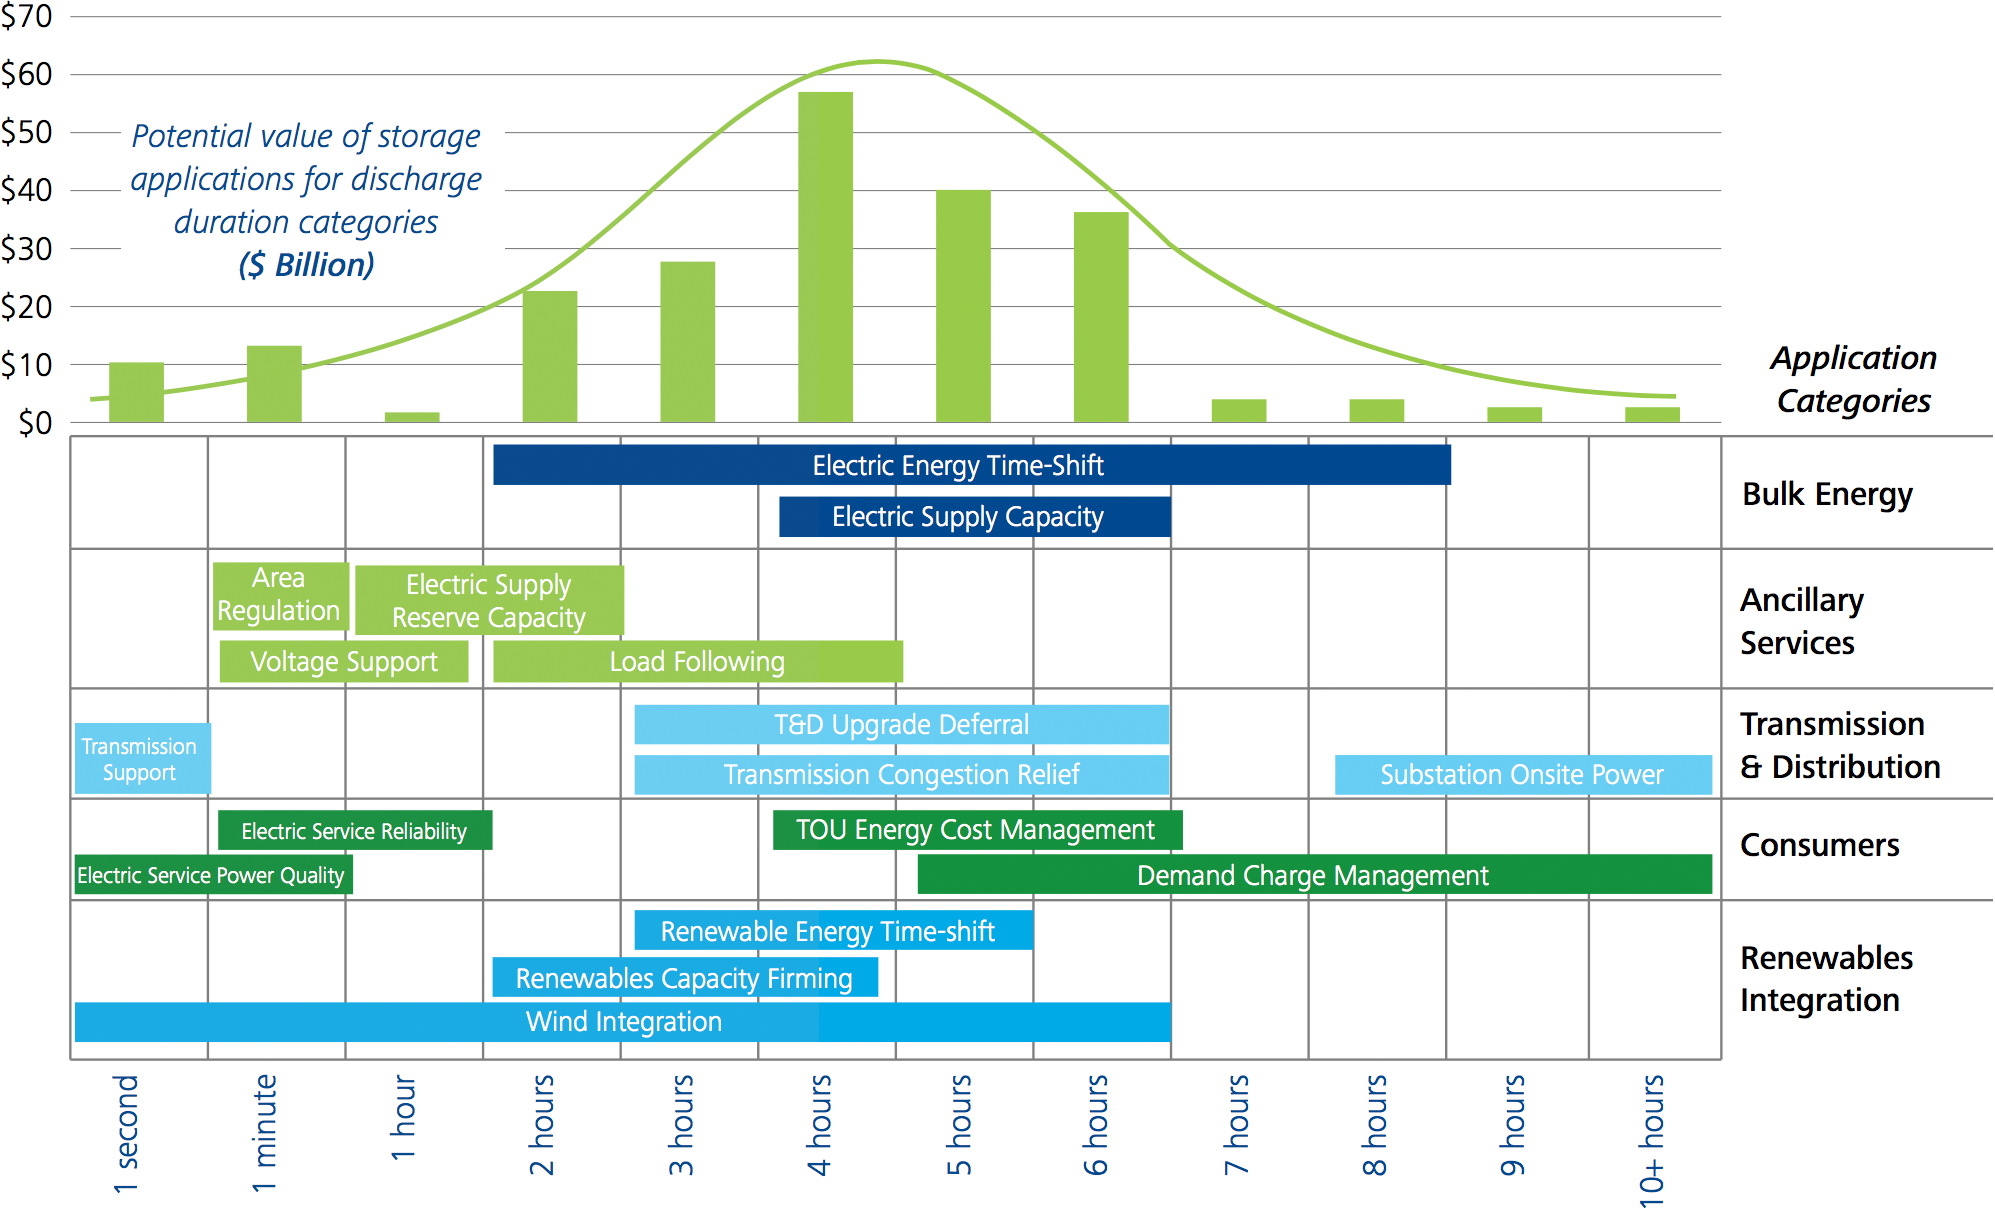
\includegraphics[width=\textwidth]{_introduction/fig/storage-financial-benefits}
	\caption{Energy storage applications and corresponding value for various discharge durations \cite{Deloitte2016}}
	\label{ch-introduction:fig:storage-financial-benefits}
\end{figure}

The idea of using energy storage in the electricity grid has been discussed for quite some time, and its important role in future energy systems has already been identified in the 70s \cite{Kalhammer1979}.
As the name suggests, electrical energy storage systems have the ability to both consume, store, and release electrical energy by converting it into a different form of energy.
Depending on the rate at which energy can be consumed and released, i.e. the system's power, as well as the amount of energy that can be stored, i.e. system's capacity, different functions can be provided.
A study for the Department Of Energy (DOE) showed that, when correctly exploited, these functions can yield direct financial benefits of \$157.56 billion over an estimated 10 year system lifecycle \cite{Eyer2010a}.
Figure \ref{ch-introduction:fig:storage-financial-benefits} shows these benefits in relation to their typical discharge period, and links them to their associated functions, too.
Here, Time Of Use (TOU) energy cost management yields the largest economic profit, yet from a historical point of view, bulk energy storage has played the most important role in the energy system.

Nowadays, storage can also tap into emerging revenue streams and perform additional functions.
As identified in several review articles \cite{Chen2009, Katsanevakis2017, Guney2017}, the key roles and applications of energy storage systems, regardless of profitability in the current market situation, can be identified as follows:

\textbf{Energy shifting - arbitrage}: This function uses the difference in energy price to yield revenue.
More specifically, as energy pricing is expected to become more dynamic and responsive to current energy demand, storage is controlled to charge when energy prices are low and discharge when energy prices are high \cite{Chen2009, Leou2012}.
Such dynamic pricing schemes are expected to emerge due to significant changes in demand at morning and evening peaks \cite{Koohi-Kamali2013}.

\textbf{Supply capacity}: In order to meet future energy demand, energy suppliers commit their resources in advance.
Doing so allows them to plan for their operation and solve the economic dispatch problem.
With increasing demand, the supply volume will have to increase, too.
However, it is predicted that energy storage can defer or even avoid investments in power plants, assuming they are sized accrodingly (i.e. several 100MW)\cite{Dobie1998}.
Bulk energy storage was the first choice to support supply capacity.
One example is pumped hydro-electric energy storage, which has seen a global growth of 127GW since 1979 \cite{Rehman2015, Barbour2015, Barbour2016}.

\textbf{Ancillary services}: These services are of interest to transmission and distribution system operators since they support the operation of their networks.
For example, load following and frequency regulation are two complementing applications of that address the imbalance between demand and supply \cite{Bevrani2011}.
In case of a severe imbalance that resulted in network outage, black start is also a function that can be supplied by energy storage \cite{Cole1995, Kashem2007}.
Since modern energy storage systems can absorb and inject both active and reactive power, they can also provide voltage support \cite{Kulkarni2005}.

\textbf{Grid stability}: To make the grid more resilient to network faults (e.g. short-circuit or loss of a large generator), or to overcome scheduled network outages, energy storage can be used as an intermittent energy source \cite{Kundur1993}.
To provide optimal operation conditions for energy generators, storage can support rotor angle stability and voltage stability by injecting active and reactive power at the point of common coupling \cite{Chakraborty2012, Kolluri2002}.
Furthermore, sub-synchronous resonance and harmonic interference can also be reduced \cite{Wang1994}.
This coupling resonance may occur between electrical and mechanical systems, can damage the mechanical structure due to repetitive stresses and strains.

\textbf{Upgrade deferral}: As already stated in Section \ref{ch-introduction:subsec:solutions-to-mitigate-impact-of-lct}, both transmission and distribution systems would have to be upgraded unless energy storage could provide network-support functions.
By deferring network upgrades, network assets will be used more efficiently, and customer disruptions will be avoided \cite{Sayer2007, Eyer2010a}.
Furthermore, in areas where the expected load has already been met and growth has levelled out, deployed energy storage is flexible enough to provide alternative functions (unlike other network assets) \cite{Huff2013}.

\textbf{Transmission charges}: In scenarios where generators are charged to use transmission systems, energy storage could take advantage of the price structure to maximise the profit from the generated energy \cite{Sayer2007, Leou2012}.

\textbf{Congestion relief}: High congestion at substations of heavily loaded transmission or distribution lines can be tackled by co-located energy storage units \cite{Saez-de-Ibarra2013a, Kulkarni2005}.
This can be achieved by e.g. shaving peak load or relaxing the energy requirements from distributed generation \cite{Reihani2016, Gerards2016d}.

\textbf{Service reliability}: In areas where a string grid connection is required to assure e.g. industry operations, an ``uninterruptible power supply'' may be required.
Traditionally, these power supplies were diesel backup generators, but modern energy storage technology can provide similar services at lower cost \cite{Schoenung2001} (particularly when including alternative revenue streams).

\textbf{Power quality}: Sub-cycle and harmonic distortions on can severely deteriorate power quality, since they can have unwanted effects on connected equipment (similar to the issue of sub-synchronous resonance at the generation side).
Energy storage with modern power electronics could be capable of providing power filtering functions that suppress those distortion \cite{Putrus2007}.
This feature could be of particular interest to LV networks in the UK, since customers are arbitrarily connected to a single phase of a three-phase network.
Therefore, the discrepancy of power quality between the phases is even larger, yet free energy storage resources could even address this issue \cite{Miret2009} (especially when considering household connected units).


\textbf{Time-of-use energy charges}: A hurdle to DSM through flexible tariffs or TOU tariffs is the reason that consumers would have to adjust their energy consumption based on external price signals, which many are do not want to do.
Energy storage could however decouple the consumer form these tariffs and allow them to continue with their normal lifestyle \cite{Khani2014}.
Additionally, when exploiting the energy price difference, storage could even supply arbitrage functions to some customers and reduce their electricity bill \cite{Nair2010a}.
For customers with local generation, e.g. PV installation, their bill can be reduction even further.
This would be done by storing the generated energy until a period of high energy prices arises.
At this time energy storage could release the energy to maximise self-consumption \cite{Luthander2016}.

\textbf{Demand charges}: Larger customers, i.e. industrial and commercial loads, are not only charged for their total energy demand, but also their for their largest continuous power demand \cite{Oudalov2007, Mackey2013}.
Therefore, a factory that may use a relatively small amount of energy over a comparatively short amount of time, is billed accordingly.
After all, the infrastructure to deliver the required power needs to be installed and maintained.
In this scenario, energy storage could reduce the intermittent power demand without significantly increasing the total energy demand, and therefore reduce demand charges for larger customers \cite{Aghaei2013}.

\textbf{Renewables integration}: Unlike traditional energy sources, renewables have are highly volatile and have limited availability.
Since their availability, i.e. for solar PV, may not align with periods of high demand, i.e. during morning and evening, arbitrage functions may be provided to maximise the use of renewable generation - i.e. renewables ``shifting'' \cite{Zakeri2015}.
Furthermore, by discharging energy storage during times of low renewable generation, e.g. due to cloud cover or varying wind, a continuous supply of energy can be assured - i.e. renewables ``smoothing''.
And lastly, if a renewable resource was committed for longer periods of time, yet the associated energy forecasts overestimated its generation capacity, storage can supply the gap to avoid balancing charges - i.e. renewables ``firming'' \cite{Chakraborty2012}.





